\documentclass[12pt,a4paper, titlepage]{article}
\usepackage{amsmath}
\usepackage{graphicx}
\usepackage{float}
\usepackage{wrapfig}
\usepackage[russian]{babel}
\usepackage[utf8]{inputenc}


\title{Лабораторная работа 4. Методы решения уравнения переноса. Вариант 2, задание 9}
\date{2021\\Апрель}
\author{Петраков Иван\\\ МФТИ\\\\\\\\\\\\\\\\\\\\}
\hoffset = 0pt
\voffset = 0pt
\textheight = 700pt
\topmargin = 0pt
\headheight = 0pt
\headsep = 0pt
\marginparwidth = 0pt
\oddsidemargin = 0pt
\textwidth = 450pt

\begin{document}

\maketitle

\subsection*{Описание задачи}
\noindent\rule{\textwidth}{1pt}
Описание задачи представлено на рисунке 1:
\begin{figure}[H]
	\centering
	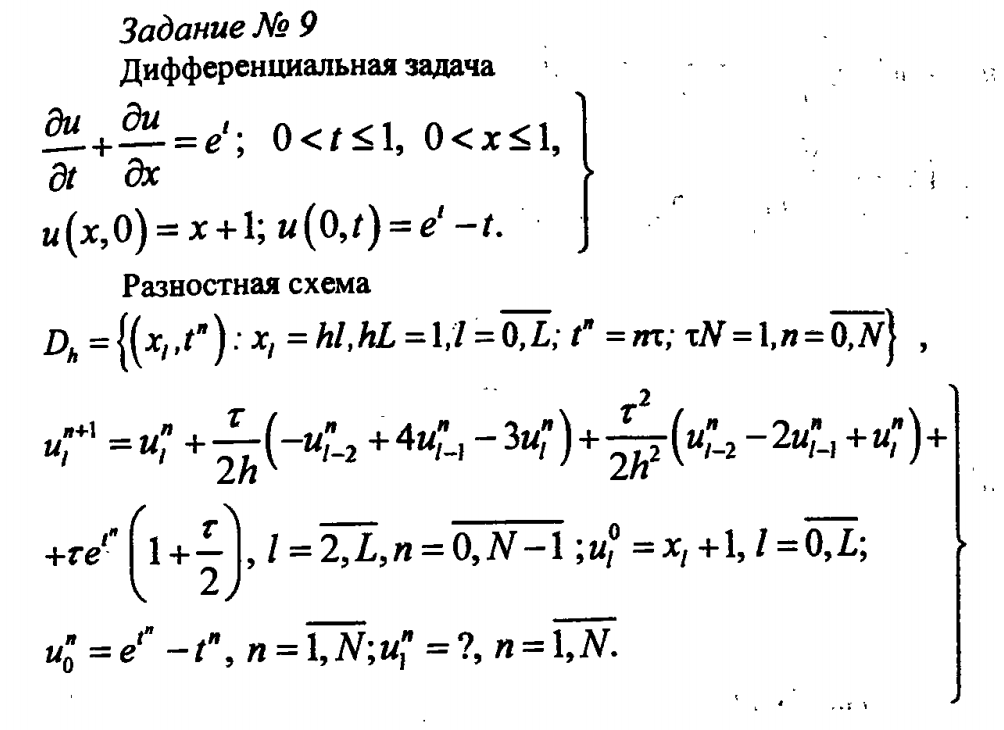
\includegraphics[width = 1.0\textwidth]{lab4_1.png}
\end{figure}

\subsection*{Аналитическое решение}
\noindent\rule{\textwidth}{1pt}

Воспользуемся предложенной научной литературой. Ищем характеристики:
\begin{equation}
dt = dx = \frac{du}{e^t}
\end{equation}
\begin{equation}
\begin{cases}
v_1(t, x) = t - x 
\\
v_2(t, u) = u - e^t
\end{cases}
\end{equation}
С помощью характеристик можно найти конечное аналитическое решение задачи:
\begin{equation}
u = e^t + x - t
\end{equation}
Подстановкой решения в изначальную задачу убеждаемся, что решение найдено верно.

\subsection*{Исследование на аппроксимацию}
\noindent\rule{\textwidth}{1pt}
Разложим след по Тейлору:
\begin{equation}
\begin{cases}
u^{n+1}_l = u^n_l + \dot{u}^n_l \tau + \ddot{u}^n_l \frac{\tau^2}{2} + O(\tau^3)
\\
u^n_{l-1} = u^n_l - u'^n_l h + u''^n_l \frac{h^2}{2} + O(h^3)
\\
u^n_{l-2} = u^n_l - u'^n_l 2h + u''^n_l 2h^2 + O(h^3)
\end{cases}
\end{equation}

Подставив в схему, получим
\begin{equation}
r = \dot{u}^n_l + \frac{\ddot{u}^n_l}{2} \tau + O(\tau^2) + u'^n_l - O(h^2) - \frac{\tau}{2} u''^n_l - \frac{\tau}{2} O(h) - e^{t^n} - \frac{e^{t^n}}{2}\tau
\end{equation}
Учтя, что 
\begin{equation}
\dot{u}^n_l + u'^n_l - e^{t^n} = 0
\end{equation}
получим второй порядок аппроксимации по h и $\tau$.
\subsection*{Исследование на устойчивость}
\noindent\rule{\textwidth}{1pt}
Воспользовавшись формулой (46) из предложенной научной литературы (либо проделав все действия заново), получим, что условие устойчивости есть 
\begin{equation}
\frac{\tau}{h} = \sigma  \leq 2
\end{equation}

\subsection*{Дополнительные условия}
\noindent\rule{\textwidth}{1pt}
Для решения задачи необходимо задать еще одно условие на $u^n_1$. Для этого разложим след по Тейлору:
\begin{equation}
u^n_{1} = u^n_0 + u'^n_0 h + u''^n_0 \frac{h^2}{2} + O(h^3)
\end{equation}
Такое разложение не нарушает наш порядок аппроксимации.
Здесь, 
\begin{equation}
\begin{cases}
u^n_0 = e^{t^n} - t^n
\\
u'^n_0 = -\dot{u}^n_0 + e^{t^n} = -e^{t^n} + e^{t^n} + 1 = 1
\\
u''^n_0 = 0
\end{cases}
\end{equation}

Отсюда получим, что 
\begin{equation}
u^n_1 = e^{t^n} - t^n + h
\end{equation}

\subsection*{Программная реализация и практические исследования}
\noindent\rule{\textwidth}{1pt}
Используя написанную мной на языке Julia1.6.0 программу, получим решение на последовательно удваеваемых сетках при $\sigma = 1.0$, что удовлетворяет условию спектральной усточивости.
\\
\\
Результаты представлены в файле \verb|6sem_lab4_solution_main.txt|.
\\
\\
Ответим на поставленные вопросы. Для ответа на вопрос про аппроксимацию построим график зависимости логарифма ошибки от логарифма шага. Тогда наклон аппроксимационной прямой в точности есть порядок сходимости.
\begin{figure}[H]
	\centering
	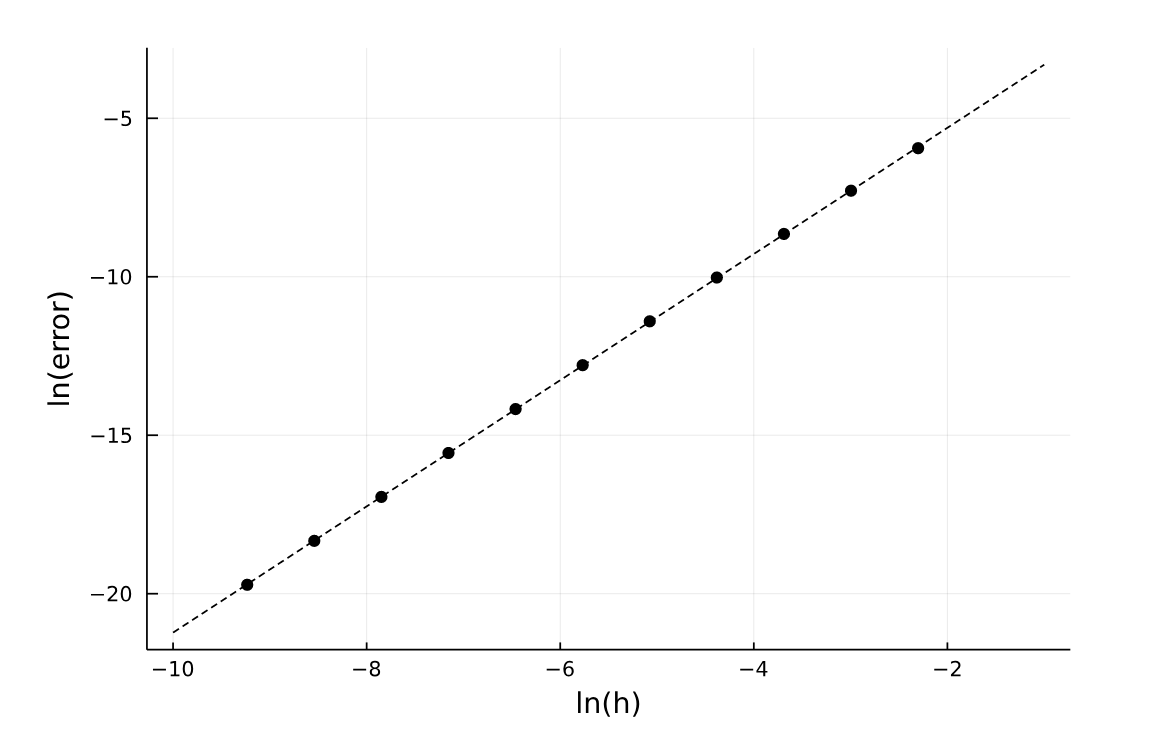
\includegraphics[width = 1.0\textwidth]{lab4_2.png}
\end{figure}
Уравнение прямой есть
\begin{equation}
fit(x) = -1.319 + 1.99084 \cdot x
\end{equation}
Отсюда получаем второй порядок аппроксимации.
\\
\\
Далее, возьмем $\sigma = 2.001$. Решение при заданной так $\sigma$ представлено в файле \verb|6sem_lab4_solution.txt|. Видно, что при нарушении условия устойчивости нарушается сходимость решения. Для данной $\sigma$ также можно построить график зависимости логарифма ошибки от логарифма шага, причем на нем достаточно хорошо наблюдается отсутствие сходимости.
\begin{figure}[H]
	\centering
	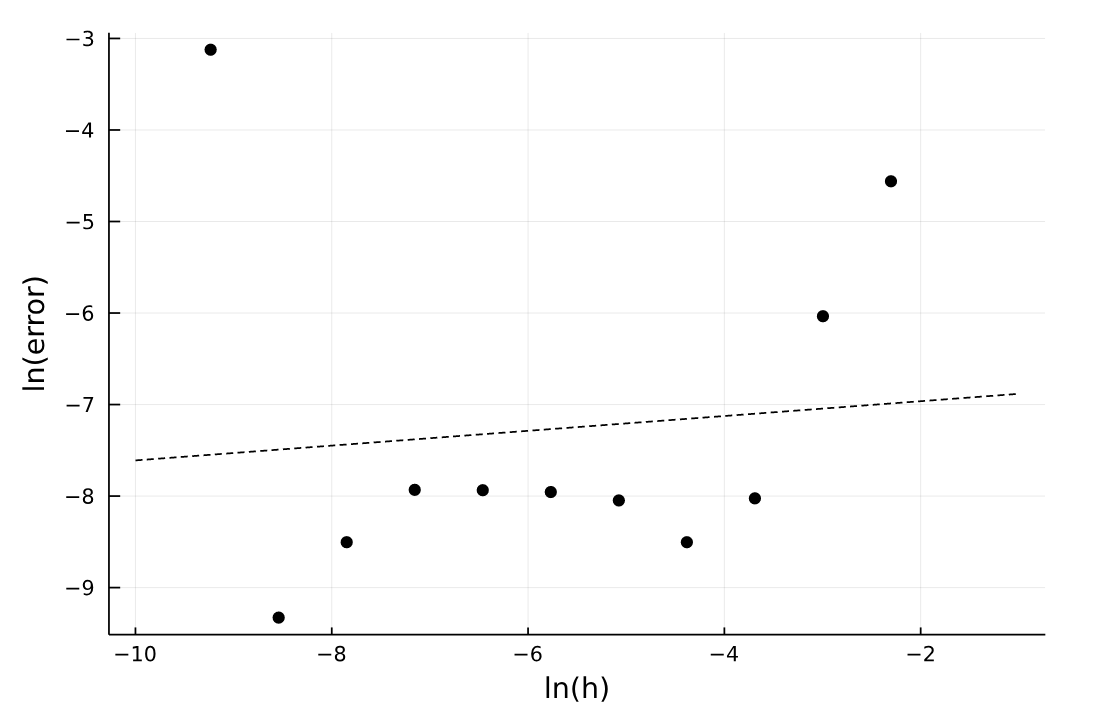
\includegraphics[width = 1.0\textwidth]{lab4_3.png}
\end{figure}
При задании дополнительных разностных уравнений мы уже, на самом деле, оставили меньшее число слагаемых, чем это предполагалось, ведь третье слагаемое, соответствующее $h^2$ занулилось. Однако, при занулении второго слагаемого, соответствующего $h$ порядок сходимости становится равным 1, что ухудшает порядок разностной схемы.
\\
\\
При изменении начальных условий результат не изменился, что связано, скорее всего, высоким порядком аппроксимации и достаточно большим количеством узлов, а зависимость от граничных условий, как было сказано выше, понижает порядок сходимости на 1.
\subsection*{Результаты и обсуждения}
\noindent\rule{\textwidth}{1pt}
В данной работе найдено аналитическое решение поставленной задачи; разностная схема исследована на аппроксимацию, причем порядок аппроксимации, полученный из теоретических соображений и программно, одинаков; разностная схема исследована на устойчивость. Также найдены дополнительные условия, позволяющие детерминировать задачу. Были проведены практические исследования на основе программной реализации решения задачи, используя высокоуровневый язык программирования - Julia.

\end{document}